\subsubsection{Rationale/Context}
Travellers might want to reserve a cabin to rest during their trip. These cabins reservations are dependent on the number of people, where the type and the price might differ.
\subsubsection{User story}
As an employee, I want to add a rental cabin with ticket reservation.
\subsubsection{Use Case}
\creator{\studentC}

\textbf{Use Case Name:} Create cabin rental reservation

\textbf{Scope:} Reservations system

\textbf{Level:} User Goal

\textbf{Primary Actor:} KOENDES Employee

\textbf{Stakeholders and Interests:} 
\begin{itemize}
\item \textit{Stakeholder:} KOENDES Employee (Wants an easy and quick process)
\item \textit{Stakeholder:} Traveller (Wants to rent a cabin with the trip reservation)
\end{itemize}

\textbf{Preconditions:} 
\begin{itemize}
\item The user is an employee and authorised to make cabin reservations and cabin rentals.
\item Travellers ticket is in process to be reserved and passengers number is filled-in.
\item There are rental cabins available for the number of travellers.
\end{itemize}

\textbf{Success Guarantee (Postconditions):}
\begin{itemize}
\item State change: The rental cabin is being added to reservation if the number of travellers is suitable for available cabin; otherwise none is added and the user gets informed.
\item Output: "Sorry, no cabin can be added to the ticket." if the number of travellers is not suitable for available cabin; otherwise "Rental cabin have been added to ticket!".
\end{itemize}

\textbf{Main Success Scenario (Basic Flow):}
\begin{enumerate}
\item The user asks the system to add a rental cabin.
\item The system reads number of passengers added to the ticket.
\item The system gets any available and suitable cabin for passengers.
\item The system calculates the price of rented cabin.
\item The system adds the cabin to the ticket.
\item The system updates the total price of ticket.
\item The system informs the user with the final result.
\end{enumerate}
Extensions:
\begin{enumerate}
\item[3a] If no available cabin is found, then move to step 6.
\end{enumerate}
\textbf{Technology And Data Variations List:} 
\begin{itemize}
    \item Passengers number: Integer
    \item Cabin Id: Integer
    \item Cabin price and Total price: Double
\end{itemize}
\textbf{Frequency of Occurrence:}
\begin{itemize}
    \item Many times per trip each day.
\end{itemize}
\subsubsection{SSD}
\creator{\studentC}\\
%\updater{Name \textsc{Surname}}
%\secondUpdater{Name \textsc{Surname}}
Considering the previous sub-sections we can create the following SSD model:\\\\
User $\rightarrow$ System: AddCabin()\hfill /* 1\\
System $\rightarrow$ System: passengersNumber = GetPasengersNumber()\hfill /* 2\\
System $\rightarrow$ System: cabinID = GetAvailableCabin(passengersNumber)\hfill /* 3\\
if cabinID is not empty\\
\phantom{x}\hspace{2ex}then\\
\phantom{x}\hspace{2ex}\phantom{x}\hspace{2ex}System $\rightarrow$ System: price = CalculatePrice(cabinID, passengersNumber)\hfill /* 4\\
\phantom{x}\hspace{2ex}\phantom{x}\hspace{2ex}System $\rightarrow$ System: addCabinToTicket(cabinID)\hfill /* 5\\
\phantom{x}\hspace{2ex}\phantom{x}\hspace{2ex}System $\rightarrow$ System: UpdateTicketPrice(price)\hfill /* 6\\
\phantom{x}\hspace{2ex}\phantom{x}\hspace{2ex}System $\rightarrow$ User: "Rental cabins have been added to ticket!"\hfill /* 7\\
else\\
\phantom{x}\hspace{2ex}System $\rightarrow$ User: "Sorry, no cabins can be added to the ticket."\hfill /* 3a $\rightarrow$ 7 \\
\newpage

%\phantom{x}\hspace{2ex}if passengerNumber == 1\\
%\phantom{x}\hspace{2ex}\phantom{x}\hspace{2ex}then price = doubleCabinPrice * 150 / 100;\\
%\phantom{x}\hspace{2ex}else\\
%\phantom{x}\hspace{2ex}\phantom{x}\hspace{2ex}then price = doubleCabinPrice;\\
%%else\\
%\phantom{x}\hspace{2ex}System $\rightarrow$ System: availableCabins = %CheckFourPersonCabins();\\
%if availableCabins\\
%\phantom{x}\hspace{2ex}then System $\rightarrow$ System: price = %CalculatePrice(passengersNumber);\hfill /* 4\\
%\phantom{x}\hspace{2ex}System $\rightarrow$ System: UpdateTicketPrice(price) \hfill /* 5\\
%\phantom{x}\hspace{2ex}System $\rightarrow$ User: "The rental cabin has been added to %ticket!"\hfill /* 6\\
%\phantom{x}\hspace{2ex}fi;\\
%else\\
%\phantom{x}\hspace{2ex}System $\rightarrow$ User: "Sorry, no cabin can be added to the %ticket."\hfill /* 6\\
%fi;\\

%\includegraphics[scale=0.9]{UC1}
\subsubsection{Grey box SD}
\creator{\studentB}
%\updater{\studentC}
\begin{figure}[H]
    \centering
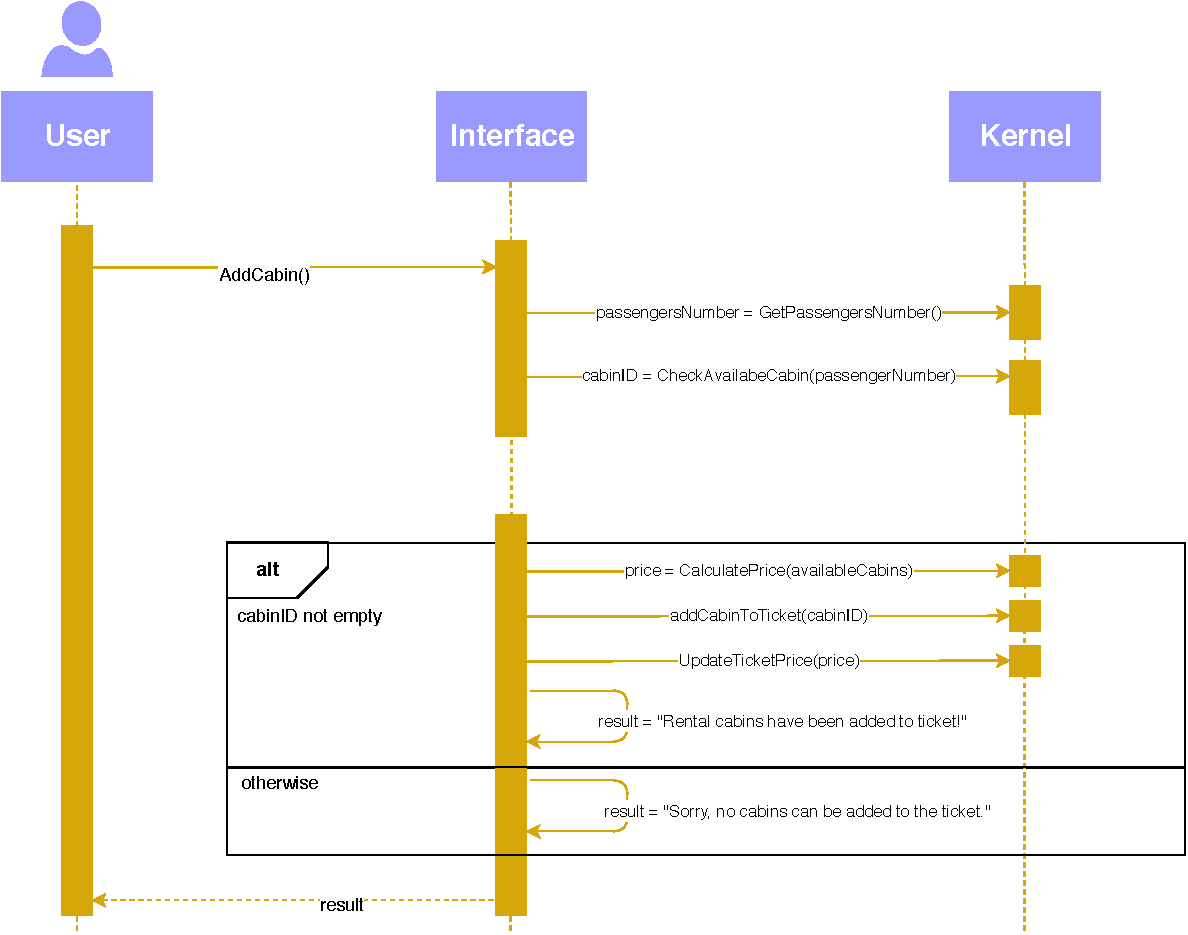
\includegraphics[scale=0.7]{Iteration_3/Files/UC5_gb.pdf}
\caption{6.5 Grey Box}
\end{figure}
 \newpage
\subsubsection{White box SD}
\creator{\studentB}
%\updater{Name \textsc{Surname}}
\newline
%\centering
\begin{figure}[H]
    \centering
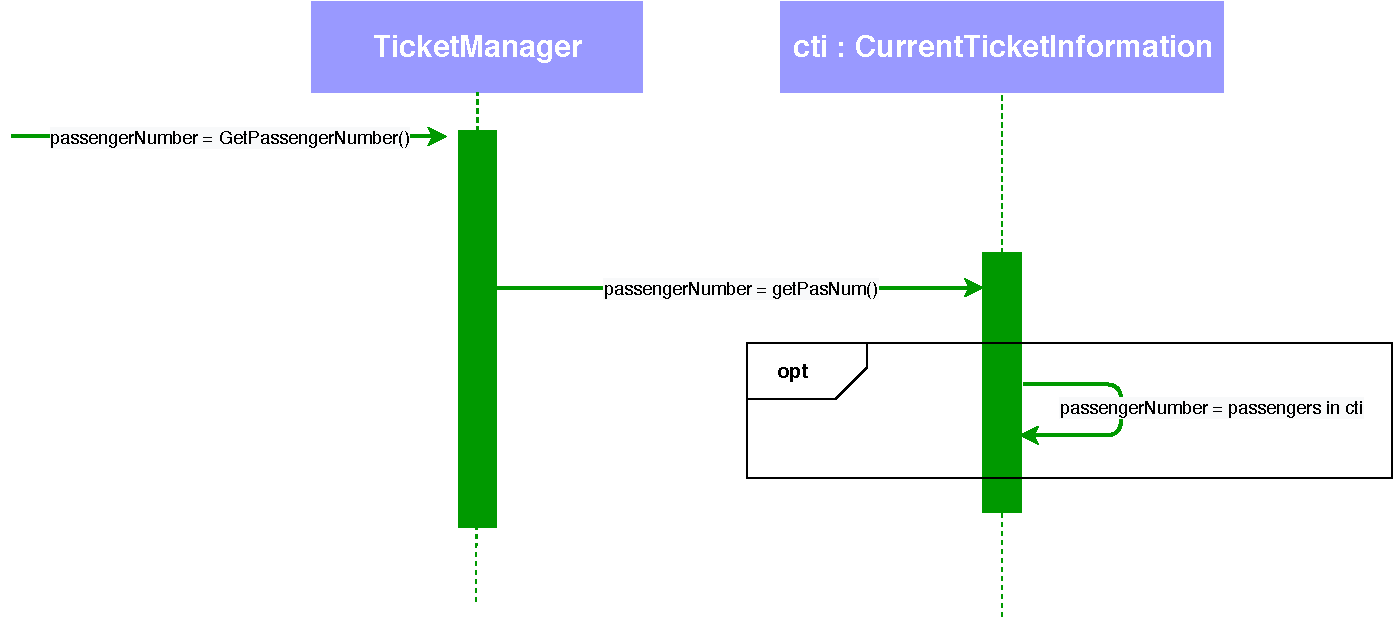
\includegraphics[scale=0.5]{Iteration_3/Files/UC5_wb1.pdf}
\end{figure}
\begin{figure}[H]
    \centering
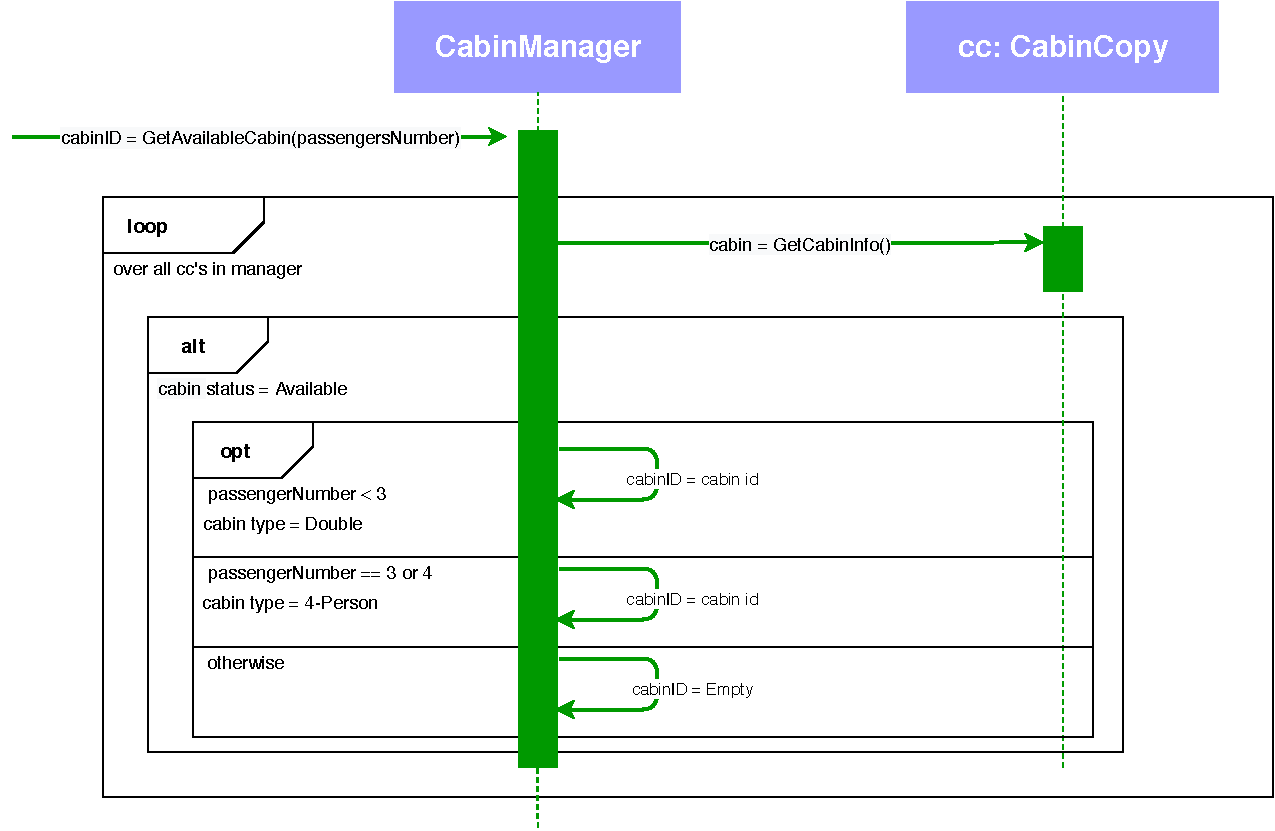
\includegraphics[scale=0.5]{Iteration_3/Files/UC5_wb2.pdf}
\end{figure}
\begin{figure}[H]
    \centering
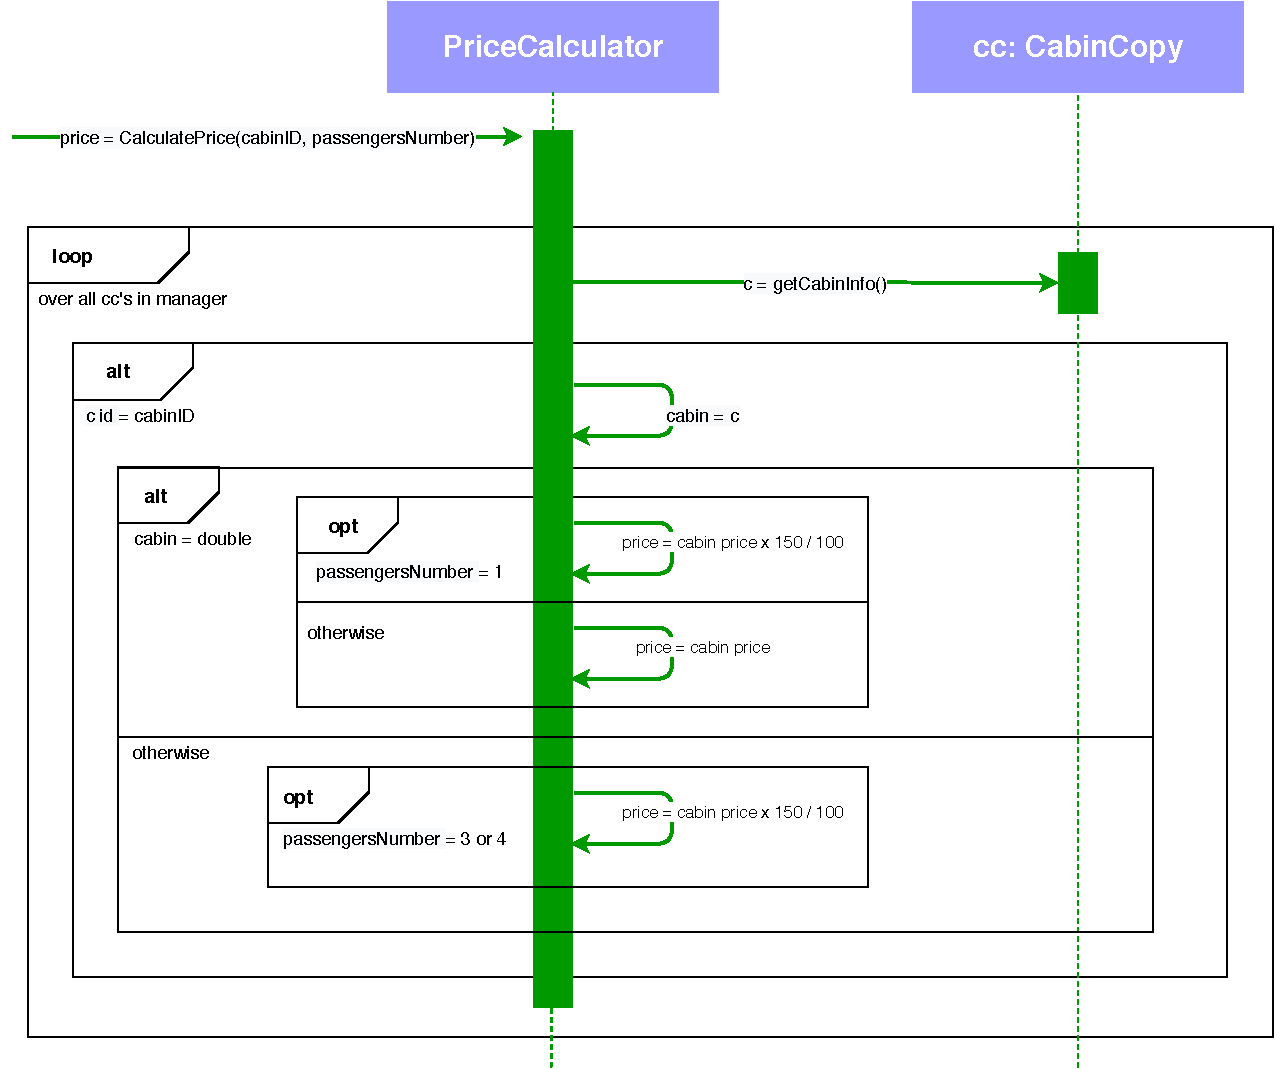
\includegraphics[scale=0.5]{Iteration_3/Files/UC5_wb3.pdf}
\end{figure}
\begin{figure}[H]
    \centering
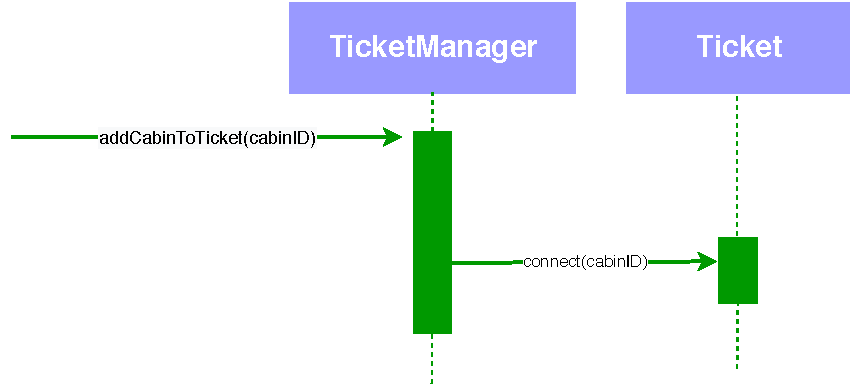
\includegraphics[scale=0.5]{Iteration_3/Files/UC5_wb4.pdf}
\end{figure}
\begin{figure}[H]
    \centering
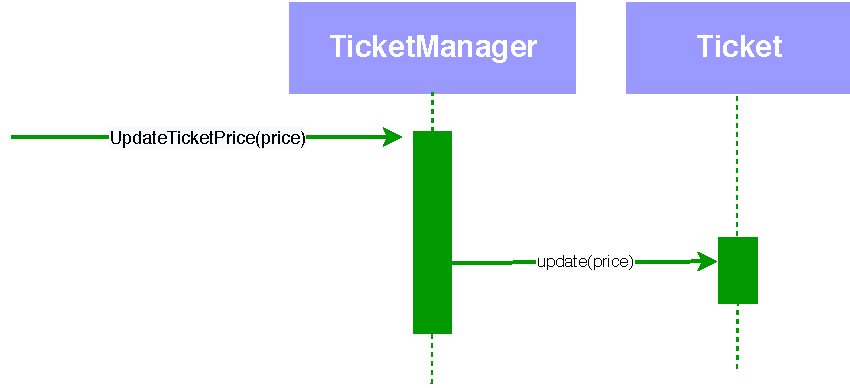
\includegraphics[scale=0.5]{Iteration_3/Files/UC5_wb5.pdf}
\end{figure}

%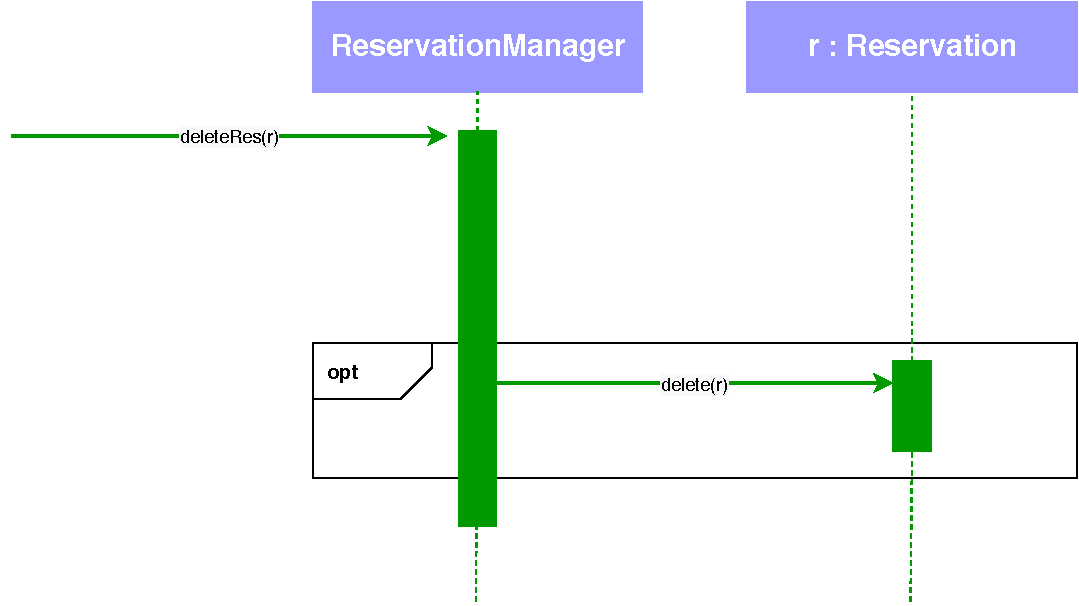
\includegraphics[scale=0.5]{Iteration_3/Files/UC3_wb2.pdf}

%\includegraphics[scale=0.9]{UC1wb.pdf}

%\subsubsection{Design Considerations}